\section{The kinematic map}\label{sec:9.2}

An aluminum film breaks Cooper pairs at $2\Delta_{\mathrm{BCS}} = \SI{0.36}{meV}$, and dark matter of \SI{0.10}{keV} can break them (\cref{we:7-al}). A silicon crystal read out through its acoustic phonons at a threshold of \SI{1}{meV} needs \SI{6.1}{keV} on its fastest longitudinal branch, sixty times more, although its threshold is less than three times higher. Its electron--hole pairs need \SI{0.333}{MeV}, and a free silicon nucleus receives the \SI{1.17}{eV} of the gap from \SI{46.8}{MeV}. A dark photon, by contrast, is absorbed in the same crystal from a mass of \SI{1.17}{eV}. These lightest masses span almost eight decades, and three things fix them: the largest laboratory speed of the halo, the energy threshold, and the shape of the dispersion of the excitation.

\subsection{The lightest mass of a channel}\label{sec:9.2-mmin}

A particle of mass $\mchi$ at the largest laboratory speed $v_{\mathrm{max}}$ deposits at most $qv_{\mathrm{max}} - q^2/2\mchi$ at momentum transfer $q$ (\cref{eq:1.3-region}). Let $E_{\mathrm{ch}}(q)$ be the lowest energy, at or above the threshold $\omega_{\mathrm{th}}$, of a final state of the channel that carries momentum $q$; we write $\omega_{\mathrm{th}}$ for the threshold $E_{\mathrm{th}}$ of \cref{sec:1.3}. The channel is open to $\mchi$ if $qv_{\mathrm{max}} - q^2/2\mchi \ge E_{\mathrm{ch}}(q)$ at some $q$. Solving for $\mchi$ and taking the most favorable $q$ gives the lightest mass of the channel,
\begin{equation}
  m_{\mathrm{min}}^{\mathrm{ch}} = \min_{q}\,\frac{q^2}{2\bigl[qv_{\mathrm{max}} - E_{\mathrm{ch}}(q)\bigr]} , \qquad qv_{\mathrm{max}} > E_{\mathrm{ch}}(q) ,
  \label{eq:9.2-mch}
\end{equation}
which is the condition \cref{eq:3.3-allowed} read as a bound on the mass. Let $\bar q$ be the momentum at which the minimum is reached. Since $E_{\mathrm{ch}}(q) \ge \omega_{\mathrm{th}}$, the bracket never exceeds $qv_{\mathrm{max}} - \omega_{\mathrm{th}}$, and the minimum over $q$ of $q^2/2(qv_{\mathrm{max}} - \omega_{\mathrm{th}})$ is $2\omega_{\mathrm{th}}/v_{\mathrm{max}}^2$. Every channel thus lies on or above the threshold mass $m_{\mathrm{min}}$ of \cref{eq:1.3-mmin}, the floor of the map, and it reaches the floor only if it has a state of energy $\omega_{\mathrm{th}}$ at $q = 2\omega_{\mathrm{th}}/v_{\mathrm{max}}$. Four shapes of $E_{\mathrm{ch}}(q)$ cover the channels of \cref{tab:9-atlas}, and absorption adds a fifth case.

\paragraph{Flat onset.} If $E_{\mathrm{ch}}(q) = E_0$ near $q = 2E_0/v_{\mathrm{max}}$, the minimum lies there and $m_{\mathrm{min}}^{\mathrm{ch}} = 2E_0/v_{\mathrm{max}}^2$, the floor with $\omega_{\mathrm{th}} \to E_0$. Optical phonons are nearly flat across the zone~\cite[Sect.~IV\,B, Eq.~(94)]{kahn2022searches}: the longitudinal optical phonon of GaAs at $\omega_{\mathrm{L}} = \SI{36.35}{meV}$ (\cref{we:5-lst}) is reached from \SI{10.35}{keV}, and the optical phonon of silicon at \SI{64.1}{meV} (\cref{sec:5.2}) from \SI{18.3}{keV}. Pair breaking in a superconductor costs $2\Delta_{\mathrm{BCS}}$ at every momentum the halo delivers, because $v_{\mathrm{F}}q \ge \omega$ there (\cref{sec:7.2}), and aluminum sits on the floor at \SI{0.10}{keV}. A core shell costs its binding energy plus the gap. The $3d$ doublet of germanium, bound by 29.2 and \SI{29.8}{eV}, opens at 8.5 and \SI{8.7}{MeV}, and the $2p$ shell of silicon, which costs $E_0 = 99.4 + \SI{1.17}{eV}$, at $2E_0/v_{\mathrm{max}}^2 = \SI{28.6}{MeV}$ (\cref{sec:10.6}, which treats ionization of the core and semicore shells). The floor is twice the least momentum at which the shell absorbs, $E_0/v_{\mathrm{max}} = \SI{38}{keV}$ (\cref{sec:3.5}), divided by $v_{\mathrm{max}}$. Two channels of gapless excitations also sit on the floor, because they do not tie the energy to one momentum: a coupling that changes at random from site to site creates a phonon of any wavevector (\cref{sec:11.6}), and two magnons share the momentum between them (\cref{sec:14.2}). At a threshold of \SI{1}{meV} both open at \SI{0.285}{keV}, 21.5 times below the acoustic edge of silicon and 5.1 times below the one-magnon edge of NiO; the map draws them as the floor line.

\paragraph{Gapless linear branch.} If the lowest state at momentum $q$ has energy $c_{\mathrm{ch}}q$, a state above threshold needs $q \ge \omega_{\mathrm{th}}/c_{\mathrm{ch}}$. The quantity minimized in \cref{eq:9.2-mch} is then $q/2(v_{\mathrm{max}} - c_{\mathrm{ch}})$, which grows with $q$, so the minimum sits at $\bar q = \omega_{\mathrm{th}}/c_{\mathrm{ch}}$ and
\begin{equation*}
  m_{\mathrm{min}}^{\mathrm{ch}} = \frac{\omega_{\mathrm{th}}}{2c_{\mathrm{ch}}(v_{\mathrm{max}} - c_{\mathrm{ch}})} \simeq \frac{\omega_{\mathrm{th}}}{2c_{\mathrm{ch}}v_{\mathrm{max}}} ,
\end{equation*}
for $c_{\mathrm{ch}} < v_{\mathrm{max}}$. For phonons this is the \emph{acoustic edge} $m_{\mathrm{min}}^{\mathrm{ac}}$, with $c_{\mathrm{ch}} = c_\nu$ the speed of the fastest branch that has a longitudinal component, since a density changes only under the component of the displacement along $\vect{q}$. It is the bound $\omega \lesssim 2c_\nu\mchi v$ of \cref{sec:1.3}~\cite[Eq.~(93)]{kahn2022searches} solved for the mass. Every acoustic edge of this chapter uses this convention; \cref{sec:11.1} also quotes the edge for the polarization-weighted inverse speed of the rate, \SI{6.39}{keV} in silicon at \SI{1}{meV}. \Cref{sec:11.1}, which computes the rate of single acoustic phonons, writes the edge as \cref{eq:11.1-edge} and finds how the rate approaches it. Compared with a flat onset of the same energy the edge is higher by $v_{\mathrm{max}}^2/4c_\nu(v_{\mathrm{max}} - c_\nu) \approx v_{\mathrm{max}}/4c_\nu$, a factor 21.5 for the longitudinal speed \SI{9.35}{km.s^{-1}} of silicon along $[111]$ (\cref{we:5-debye}). The reason is momentum. A phonon of energy $\omega_{\mathrm{th}}$ carries $\omega_{\mathrm{th}}/c_\nu$, and the dark matter hands over that much momentum by backscattering, at $q = 2\mchi(v_{\mathrm{max}} - c_\nu)$, where it gives up a fraction $4c_\nu/v_{\mathrm{max}}$ of its kinetic energy. The magnons of an antiferromagnet are linear near their gapless points, with a velocity $c_{\mathrm{M}}$ near $10^{-4}$ (\cref{we:7-nio}), some four times the fastest sound speed of silicon. In NiO the fastest magnon velocity is $c_{\mathrm{M}} = 1.36\times10^{-4}$, and the edge at a \SI{5}{meV} threshold is \SI{7.3}{keV} (\cref{sec:14.1}, which computes the one-magnon rate of NiO).

If $c_{\mathrm{ch}} \ge v_{\mathrm{max}}$, no mass reaches the channel: the deposit $qv_{\mathrm{max}} - q^2/2\mchi$ lies below $c_{\mathrm{ch}}q$ at every $q$. Two channels inside populated cells of \cref{tab:9-atlas} are closed this way to elastic scattering. The bulk plasmon of silicon, with the quadratic dispersion $\omega_{\mathrm{pl}}^2 = \omega_p^2 + \tfrac35q^2v_{\mathrm{F}}^2$ of \cref{sec:4.5}, has a phase velocity $\omega_{\mathrm{pl}}(q)/q$ that falls to $9.2\times10^{-3}$, or $3.5\,v_{\mathrm{max}}$, where it meets the pair continuum at \SI{2.24}{keV} (\cref{sec:10.3}, electron-gas models and the plasmon), so halo dark matter never excites it. The narrow-gap III--V semiconductors, however, are massive Dirac cones with $v_{\mathrm{D}} \approx 1.8\,v_{\mathrm{max}}$ (\cref{sec:7.3}), and their pairs are closed to scattering at every mass, while absorption stays open.

\paragraph{Gapped linear branch.} A branch $E_{\mathrm{ch}}(q) = (c_{\mathrm{ch}}^2q^2 + E_0^2)^{1/2}$ interpolates between the two shapes: flat for $c_{\mathrm{ch}} \ll v_{\mathrm{max}}$, closed for $c_{\mathrm{ch}} \ge v_{\mathrm{max}}$. The pair continuum of a Dirac material has this form with $c_{\mathrm{ch}} = v_{\mathrm{D}}$ and $E_0 = 2\Delta_{\mathrm{D}}$ (\cref{eq:7.3-edge}). For ZrTe$_5$, with the half-gap $\Delta_{\mathrm{D}} = \SI{11.8}{meV}$ of the measured crystal structure (the relaxed cell of \cref{we:7-zrte5} gives \SI{15.6}{meV}) and $v_{\mathrm{D}}/v_{\mathrm{max}}$ between 0.17 and 0.42 along its principal axes (\cref{sec:16.1}), the lightest mass is \SI{7.1}{keV}, with $\vect{q}$ along the slow axis; along the other two axes it is 9.0 and \SI{9.6}{keV}. A flat continuum would give $4\Delta_{\mathrm{D}}/v_{\mathrm{max}}^2 = \SI{6.72}{keV}$, and the isotropic cone with the geometric-mean velocity $7.9\times10^{-4}$, which \cref{sec:16.1} uses for the average over orientations, gives \SI{8.0}{keV}. A magnon with a gap has the same shape. Single-ion anisotropy lifts the gapless mode of an antiferromagnet to the antiferromagnetic resonance, the geometric mean of the anisotropy energy and twice the exchange energy of a spin (\cref{eq:14.3-afmr}). It lies at \SI{1.1}{meV} in MnF$_2$ (\cref{sec:14.3}, absorption into magnons). In NiO the anisotropy gaps the two branches differently: far-infrared absorption places one zone-center magnon at \SI{4.54}{meV}, and the other lies near \SI{0.6}{meV} (\cref{sec:14.1}). Since $c_{\mathrm{M}} \ll v_{\mathrm{max}}$, a gapped magnon sits within a percent of the flat value: \SI{1.30}{keV} for the mode at \SI{4.54}{meV}.

\paragraph{Offset minimum.} In an indirect-gap crystal $E_{\mathrm{ch}}(q)$ comes down to $\Eg$ only near the valley momentum $k_{\mathrm{c}}$ (\cref{eq:3.3-Emin}), while the floor needs $\Eg$ at $q = 2\Eg/v_{\mathrm{max}}$, \SI{0.88}{keV} in silicon against $k_{\mathrm{c}} = \SI{1.94}{keV}$. The minimum of \cref{eq:9.2-mch} lies between the floor and the mass that deposits $\Eg$ at exactly $k_{\mathrm{c}}$: between 0.333 and \SI{0.474}{MeV} in silicon, and between 0.212 and \SI{0.420}{MeV} in germanium (\cref{we:3-kc,we:3-mmin}). A phonon can take up the mismatch of momentum cheaply. At the floor the dark matter delivers $\bar q \approx \SI{0.89}{keV}$, and the phonon supplies the rest of $k_{\mathrm{c}}$, \SI{1.06}{keV}, where a transverse acoustic phonon costs \SI{14.8}{meV}. Absorption brings no momentum and needs a phonon at $k_{\mathrm{c}}$ itself, at \SI{18.3}{meV}; that is why its threshold, \SI{1.1728}{eV}, lies above the bound pair plus \SI{15}{meV}. This places the phonon-assisted onset just above the floor: \SI{0.3332}{MeV} for a pair bound to an exciton and \SI{0.3374}{MeV} for a free pair in silicon, and 0.2119 to \SI{0.2141}{MeV} in germanium (\cref{sec:13.1}, which derives both thresholds of an indirect gap). Without a phonon the edge of silicon lies at 0.405 to \SI{0.408}{MeV} (\cref{sec:13.9}, which collects the silicon window), and between the two edges dark matter creates pairs together with a phonon or not at all. For germanium the zero-phonon edge is an estimate. A parabolic pair on the L axis gives \SI{0.32}{MeV}. The minimum need not lie on the axis, however, and the heavy hole is warped and mixed by spin--orbit coupling, so the value bounds the edge in neither direction (\cref{sec:13.1}). A direct gap does not remove the problem. GaAs has both band edges at $\mathrm{\Gamma}$, but a pair there that absorbs the \SI{1.15}{keV} at which $\Eg = \SI{1.52}{eV}$ is deposited gains a kinetic energy comparable to the gap. Its phonon-assisted onset, 0.433 to \SI{0.436}{MeV}, sits at the floor, and its first zero-phonon states are those of the L valleys at \SI{1.815}{eV}, which open between 0.517 and \SI{0.560}{MeV} (\cref{sec:13.1}).

\paragraph{Quadratic branch.} A free nucleus recoils with $E = q^2/2M$, and \cref{eq:9.2-mch} reproduces the largest recoil energy $E_R^{\mathrm{max}} = 2\mu_{\chi N}^2v_{\mathrm{max}}^2/M$ of \cref{eq:1.3-ERmax}. The lightest mass that deposits $\omega_{\mathrm{th}}$ solves $E_R^{\mathrm{max}}(\mchi) = \omega_{\mathrm{th}}$, which for $\mchi \ll M$ is $\mchi \simeq (M\omega_{\mathrm{th}}/2)^{1/2}/v_{\mathrm{max}}$: it grows as the square root of the threshold. The recoil is free once it exceeds several phonon energies, and how many depends on the quantity compared (\cref{we:9-place}). \Cref{sec:11.4}, which treats nuclear recoil in the impulse approximation, replaces the sum over phonon numbers by the impulse Gaussian at four mean phonon energies, \SI{0.164}{eV} in silicon, reached from \SI{17.5}{MeV}. For germanium the estimate is \SI{21.3}{MeV} (\cref{sec:17.1}, which compares the scattering channels of silicon, germanium and GaAs). The map and the plane of \cref{sec:9.3} use this onset. Below the onset mass a nucleon coupling excites several phonons or one, whose kinematics are the shapes above. The Migdal effect, in which a nuclear recoil also excites the electrons, lets the crystal absorb the momentum while the electrons take the energy, so it opens at the floor of the gap, \SI{0.333}{MeV} in silicon (\cref{sec:17.1}).

\paragraph{Absorption.} A boson of mass $m_\phi$ brings the energy $m_\phi$ and the momentum $m_\phi v \le 2.65\times10^{-3}\,m_\phi$ (\cref{sec:8.2-absorption}). The lightest mass a target absorbs is the lowest energy of an excitation at $q \simeq 0$ that the coupling reaches:
\begin{equation}
  m_\phi = \omega , \qquad q = m_\phi v \simeq 0 .
  \label{eq:9.2-abs}
\end{equation}
At equal deposited energy, absorption reaches masses $2/v_{\mathrm{max}}^2 = 2.85\times10^5$ times lighter than scattering, five and a half decades. The condition $q \simeq 0$ also selects the excitations: no acoustic phonon absorbs (\cref{sec:9.1-empty}), and across the indirect gap of silicon or germanium a phonon must again supply the momentum (\cref{sec:3.3}). Electronic absorption in cold silicon begins at \SI{1.1728}{eV}, where a pair bound by \SI{14.7}{meV} is created together with a transverse acoustic phonon (\cref{sec:13.8}, exciton replicas and bosonic absorption). No single phonon of silicon absorbs at all (\cref{sec:9.1-empty}). GaAs absorbs a dark photon in its longitudinal optical phonon at \SI{36.35}{meV} (\cref{sec:11.8}), aluminum from $2\Delta_{\mathrm{BCS}}$ (\cref{sec:15.4}, absorption in superconductors and metals), and ZrTe$_5$ from $2\Delta_{\mathrm{D}} = \SI{23.6}{meV}$ (\cref{sec:16.1}). In a ferromagnet the uniform precession of the spins absorbs at a frequency tuned by an applied field at \SI{116}{\micro eV} per tesla, from a few \si{\micro eV} to about a meV (\cref{sec:14.3}). The normal modes of the detector body, at MHz in a millimeter crystal, continue the line down to the neV range (\cref{sec:11.8}).

\subsection{Edges of five targets}\label{sec:9.2-map}

\Cref{fig:9-kinmap}a draws the lightest mass of every channel against its threshold, and \cref{tab:9-edges} lists the edges of the five targets. On logarithmic axes the absorption line $m_\phi = \omega$ and the floor $2\omega_{\mathrm{th}}/v_{\mathrm{max}}^2$ are parallel. The acoustic edges and the magnon edge run parallel to both, above the floor by $v_{\mathrm{max}}/4c_{\mathrm{ch}}$, while the free-recoil curves rise with half the slope; they would meet the floor only at $\mchi = M$, where an elastic collision can transfer the whole kinetic energy. The scattering channels fall into three groups of mass. Collective modes and the pairs of small-gap materials, with energies from a fraction of a meV to tens of meV, open between \SI{0.1}{keV} and \SI{20}{keV}. Electron--hole pairs across gaps near an eV open between 0.2 and \SI{0.6}{MeV}, the region enlarged in \cref{fig:9-kinmap}b. Free nuclear recoils and core shells need about \SI{10}{MeV} or more.

\begin{figure}[tbp]
  \centering
  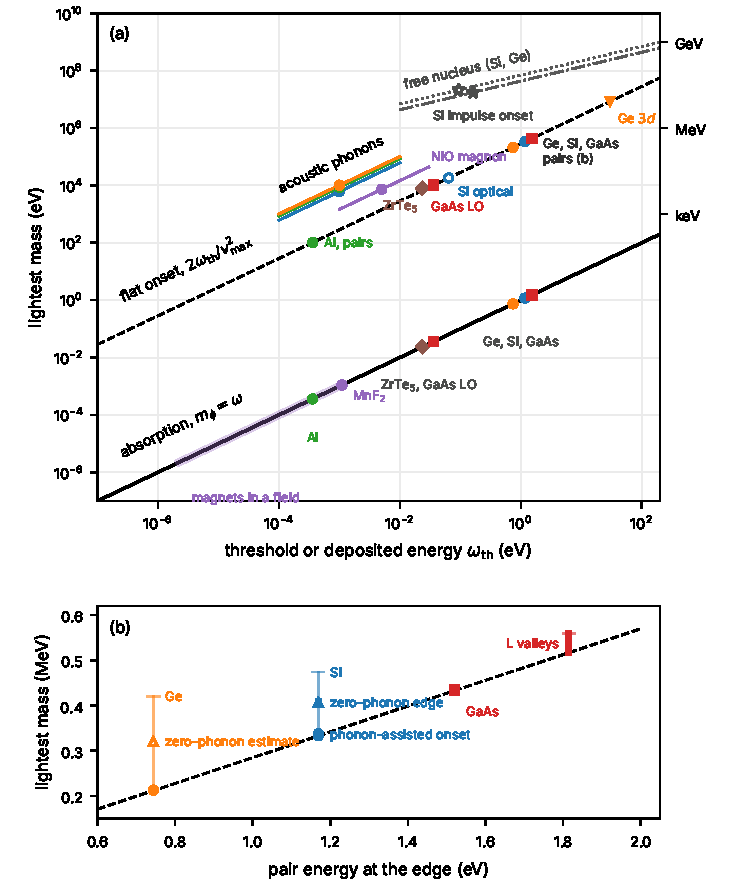
\includegraphics[width=0.78\linewidth]{figures/ch09/fig9_1.pdf}
  \caption{The kinematic map at $v_{\mathrm{max}} = \SI{794.5}{km.s^{-1}}$ (\cref{tab:1-shm}), elastic scattering. (a)~Lightest dark-matter mass of each scattering channel and lightest absorbed boson mass, against the threshold or the energy of the excitation. Solid black: absorption, $m_\phi = \omega$. Dashed: the floor $2\omega_{\mathrm{th}}/v_{\mathrm{max}}^2$, reached by flat onsets. Colored lines: acoustic edges $\omega_{\mathrm{th}}/[2c_\nu(v_{\mathrm{max}} - c_\nu)]$ for the fastest longitudinal speeds of silicon (\SI{9.35}{km.s^{-1}}, lowest), aluminum (\SI{6.67}{km.s^{-1}}, along [111]) and germanium (\SI{5.60}{km.s^{-1}}), drawn from 0.1 to \SI{10}{meV}, with their values at \SI{1}{meV} (dots); purple, the magnon edge of NiO with $c_{\mathrm{M}} = 1.36\times10^{-4}$, with its value at \SI{5}{meV}. Gray: largest free recoil of a silicon (dash-dotted) and germanium (dotted) nucleus, with the impulse onsets (stars; open: estimate). Points on the floor: aluminum pair breaking, the optical phonons of GaAs (square) and silicon (open circle), the germanium $3d$ shell; diamond and bar: ZrTe$_5$, isotropic cone and principal axes (the lowest end, \SI{7.1}{keV}, is its lightest mass). Points on the absorption line: aluminum, MnF$_2$, ZrTe$_5$, GaAs (optical phonon), germanium, silicon and GaAs (electrons); band: the uniform mode of a magnet tuned by a field. (b)~Electron--hole pairs. Filled circles and squares: phonon-assisted onsets; thick bars and filled triangle: zero-phonon edges (silicon, GaAs L valleys); open triangle: germanium zero-phonon estimate, which bounds the edge in neither direction; thin lines: from the floor to the mass that deposits the gap at exactly the valley momentum. Values and their sources in \cref{tab:9-edges}.}
  \label{fig:9-kinmap}
\end{figure}

\begin{table}[tbp]
  \caption{Channel edges of five targets: the lightest mass that reaches each channel in elastic scattering, and the lightest absorbed boson mass, at $v_{\mathrm{max}} = \SI{794.5}{km.s^{-1}}$. Masses in MeV unless marked. ``--'': no such channel; ``n.e.'': not evaluated in this book. The last column gives the section where each value is computed. Entries without a section there are computed here from \cref{eq:9.2-mch}: the aluminum acoustic edge, with the speed \SI{6.67}{km.s^{-1}} along [111] from the zero-temperature elastic constants and density of \cref{sec:20.3}; the floor of ZrTe$_5$; and the silicon $2p$ edge. Estimates are marked.}
  \label{tab:9-edges}
  \centering\footnotesize\setlength{\tabcolsep}{2.5pt}
  \begin{tabular}{@{}>{\raggedright\arraybackslash}p{0.18\linewidth}>{\raggedright\arraybackslash}p{0.12\linewidth}>{\raggedright\arraybackslash}p{0.12\linewidth}>{\raggedright\arraybackslash}p{0.13\linewidth}>{\raggedright\arraybackslash}p{0.08\linewidth}>{\raggedright\arraybackslash}p{0.12\linewidth}>{\raggedright\arraybackslash}p{0.10\linewidth}@{}}
    \toprule
    Channel & Si & Ge & GaAs & Al & ZrTe$_5$ & Section \\
    \midrule
    Floor of the gap, $2\Eg/v_{\mathrm{max}}^2$ & 0.333 & 0.212 & 0.433 & -- & \SI{6.72}{keV} ($4\Delta_{\mathrm{D}}/v_{\mathrm{max}}^2$) & \cref{sec:1.3} \\
    Pairs with a phonon (onset) & 0.3332 (exciton), 0.3374 (free pair) & 0.2119--0.2141 & 0.433--0.436 & -- & n.e. & \cref{sec:13.1} \\
    Pairs without a phonon & 0.405--0.408 & $\approx 0.32$; estimate & 0.517--0.560 (L valleys) & -- & \SI{7.1}{keV} (slow axis; 9.0, \SI{9.6}{keV} along the others) & \cref{sec:13.9,sec:13.1,sec:16.1} \\
    Pair breaking, $2\Delta_{\mathrm{BCS}}$ & -- & -- & -- & \SI{0.10}{keV} & -- & \cref{sec:7.2} \\
    One acoustic phonon, $\omega_{\mathrm{th}} = \SI{1}{meV}$ & \SI{6.1}{keV} & \SI{10.2}{keV} & 10.3--\SI{12.3}{keV} (computed tensors) & \SI{8.6}{keV} & n.e. & \cref{sec:11.1,sec:17.1,sec:17.6} \\
    One optical phonon & \SI{18.3}{keV} & n.e. & \SI{10.35}{keV} & -- & n.e. & \cref{sec:17.3,sec:11.2} \\
    Core shell & 28.6 ($2p$) & 8.5--8.7 ($3d$) & n.e. & n.e. & n.e. & \cref{sec:10.6} \\
    Free nuclear recoil (impulse onset) & 17.5 & 21.3; estimate & n.e. & n.e. & n.e. & \cref{sec:11.4,sec:17.1} \\
    Absorption, lowest $m_\phi$ & \SI{1.1728}{eV} (pairs with a phonon) & $\approx\SI{0.74}{eV}$ with a phonon, \SI{0.89}{eV} without & \SI{36.35}{meV} (optical phonon); \SI{1.52}{eV} (pairs) & \SI{0.36}{meV} & \SI{23.6}{meV} & \cref{sec:13.8,sec:3.3,sec:11.8,sec:15.4,sec:16.1} \\
    \bottomrule
  \end{tabular}
\end{table}

Inside the first group the map orders the targets by stiffness and by gap. At a common threshold of \SI{1}{meV} the acoustic edge falls as the longitudinal sound speed rises, from \SI{6.1}{keV} in silicon to 10.3 to \SI{12.3}{keV} in GaAs, whose elastic tensor is a computed one (\cref{tab:9-edges}; \cref{sec:17.6}, which ranks the targets when their inputs are uncertain). Diamond reaches \SI{3.1}{keV} (\cref{sec:17.5}, figures of merit of the channels). A flat mode competes with an acoustic one read out at a much lower threshold. The optical phonon of GaAs at \SI{36.35}{meV} opens at \SI{10.35}{keV}, the acoustic edge that silicon has at a threshold of \SI{1.7}{meV}. The pairs of ZrTe$_5$ across \SI{23.6}{meV} open at \SI{7.1}{keV}, the silicon edge at \SI{1.16}{meV}; and the NiO magnon at \SI{5}{meV} opens at \SI{7.3}{keV}, the silicon edge at \SI{1.2}{meV}.

In the second group the gap sets the order, germanium, silicon and GaAs, and every crystal of the three has a band above its floor in which pairs need a phonon. In germanium the upper end of that band is not known, and in GaAs it ends where the L valleys open. A detector that counts pairs reaches its floor through phonon-assisted scattering, the process that \cref{chap:13} treats. In the third group the square-root growth of the free-recoil mass makes the nuclear edge of germanium higher than that of silicon by only $(M_{\mathrm{Ge}}/M_{\mathrm{Si}})^{1/2}$ at equal recoil energy.

The map ranks reach, not rate. At the edge itself only particles at $v_{\mathrm{max}}$, moving along the right direction, contribute, and the rate vanishes (\cref{sec:1.3-edge}); a reach curve turns up steeply as the mass approaches the edge from above. For one acoustic phonon, \cref{sec:11.1} finds that the rate comes within \SI{10}{\percent} of its value for heavy particles only above 44 times the edge. Comparing two targets near their edges therefore needs the rates of the chapters that follow.

\begin{workedexample}{The acoustic edge of silicon at a threshold of 1 meV}\label{we:9-acoustic}
The fastest longitudinal branch of silicon runs along $[111]$, with $c_{\mathrm{LA}} = \SI{9.35}{km.s^{-1}}$ from the measured elastic constants (\cref{we:5-debye}). In units of the speed of light, $c_{\mathrm{LA}} = 9.35/299792 = 3.119\times10^{-5}$, and $v_{\mathrm{max}} = 794.5/299792 = 2.650\times10^{-3}$. A phonon of energy $\omega_{\mathrm{th}} = \SI{1}{meV}$ on this branch carries
\begin{equation*}
  \bar q = \frac{\omega_{\mathrm{th}}}{c_{\mathrm{LA}}} = \frac{\SI{e-3}{eV}}{3.119\times10^{-5}} = \SI{32.1}{eV} .
\end{equation*}
This is $0.014\,(2\pi/a)$, with $2\pi/a = \SI{2.28}{keV}$, deep in the linear part of the branch, where the edge needs slopes that obey the acoustic sum rule (\cref{sec:5.2}). With $v_{\mathrm{max}} - c_{\mathrm{LA}} = 2.619\times10^{-3}$,
\begin{equation*}
  m_{\mathrm{min}}^{\mathrm{ac}} = \frac{\SI{e-3}{eV}}{2 \times 3.119\times10^{-5} \times 2.619\times10^{-3}} = \SI{6.12}{keV} .
\end{equation*}
The floor at the same threshold is $2\omega_{\mathrm{th}}/v_{\mathrm{max}}^2 = \SI{0.285}{keV}$. A particle of \SI{6.12}{keV} at $v_{\mathrm{max}}$ has \SI{21.5}{meV} of kinetic energy and could give all of it to a target that absorbs the momentum $\mchi v_{\mathrm{max}} = \SI{16.2}{eV}$, but a phonon with that momentum carries only \SI{0.51}{meV}. To create the \SI{1}{meV} phonon the particle must reverse its direction, giving $2\mchi(v_{\mathrm{max}} - c_{\mathrm{LA}}) = \SI{32.1}{eV}$, and it keeps \SI{20.5}{meV} of its energy. Along $[100]$ the transverse speed \SI{5.84}{km.s^{-1}} of \cref{we:5-debye} would give \SI{9.76}{keV}, but a transverse phonon along a symmetry axis carries no density and is not excited by a density coupling. The edge scales linearly with the threshold, \SI{0.61}{keV} at \SI{0.1}{meV} and \SI{61}{keV} at \SI{10}{meV}, as long as $\bar q$ stays in the linear part of the branch; at \SI{10}{meV} it is already $0.14\,(2\pi/a)$. \Cref{sec:11.1} evaluates the rate near this edge with all branches and directions.
\end{workedexample}

\subsection{Dependence on the halo}\label{sec:9.2-halo}

Every scattering edge moves with $v_{\mathrm{max}} = v_{\mathrm{esc}} + v_{\mathrm{E}}^{\mathrm{ref}}$, but not by the same amount. At the minimum of \cref{eq:9.2-mch} either the derivative with respect to $q$ vanishes or $q$ sits on a constraint that does not depend on $v_{\mathrm{max}}$. Differentiating then leaves the explicit dependence alone:
\begin{equation}
  \frac{\dd\ln m_{\mathrm{min}}^{\mathrm{ch}}}{\dd\ln v_{\mathrm{max}}} = -\frac{\bar qv_{\mathrm{max}}}{\bar qv_{\mathrm{max}} - E_{\mathrm{ch}}(\bar q)} .
  \label{eq:9.2-halo}
\end{equation}
The ratio on the right compares the largest energy the particle could deposit at $\bar q$ with what is left after the excitation is paid. For a flat onset $\bar q = 2E_0/v_{\mathrm{max}}$, half of $\bar qv_{\mathrm{max}}$ goes into the excitation, and the exponent is $-2$, the halo dependence of the floor in \cref{sec:1.3}. For a gapless linear branch $\bar q = \omega_{\mathrm{th}}/c_{\mathrm{ch}}$ and the exponent is $-v_{\mathrm{max}}/(v_{\mathrm{max}} - c_{\mathrm{ch}})$, which is $-1.012$ for silicon: the acoustic edge scales as $1/v_{\mathrm{max}}$, not $1/v_{\mathrm{max}}^2$, because the excitation takes the small fraction $c_\nu/v_{\mathrm{max}}$ of $\bar qv_{\mathrm{max}}$. A free nucleus gives $-1$ for $\mchi \ll M$, from $\mchi \simeq (M\omega_{\mathrm{th}}/2)^{1/2}/v_{\mathrm{max}}$. At a stationary minimum, where the derivative with respect to $q$ vanishes, $\bar qv_{\mathrm{max}} = 2E_{\mathrm{ch}} - \bar qE_{\mathrm{ch}}'$. A branch that rises there takes more than half of $\bar qv_{\mathrm{max}}$, and the exponent exceeds 2 in magnitude: $-2.37$ for the isotropic cone of ZrTe$_5$, and $-2.12$ to $-2.74$ along its axes. A branch that falls there, as on the way to an indirect valley, gives less than 2. The gapless linear branch also rises, but its minimum sits on the constraint $q \ge \omega_{\mathrm{th}}/c_{\mathrm{ch}}$, not at a stationary point. Absorption, \cref{eq:9.2-abs}, does not depend on the halo at all.

The halo matters at the level of a few percent. The uncertainty of \SI{25}{km.s^{-1}} in the escape speed moves the floor and every flat onset by \SI{6.3}{\percent} (\cref{sec:1.3}; exactly \SI{-6.0}{\percent} and \SI{+6.6}{\percent}), and to first order the acoustic edge of silicon by \SI{3.2}{\percent}, the free-recoil edges by \SI{3.1}{\percent} and the Dirac edge of ZrTe$_5$ by \SI{7.4}{\percent}. Over the year the acoustic edge of silicon moves by \SI{-2.0}{\percent} in June and \SI{+1.7}{\percent} in December, about half the shift of the floor. A different halo thus shifts the map without reordering channels of the same shape, but it changes the ratio between a flat and a linear edge by about $\delta\ln v_{\mathrm{max}}$. \Cref{sec:17.3}, which treats inelastic scattering into collective modes, finds that a splitting of \SI{10}{meV} moves the phonon and magnon edges by 12 to \SI{28}{\percent} and the electronic edge of silicon by \SI{1}{\percent} (\cref{tab:17-endo}). An exothermic splitting larger than the excitation energy removes the edge altogether, as \cref{sec:1.3} found for the threshold mass.
